\section{Introduction}

\iftoggle{plan}{
  20 columns papers :

  \begin{center}
    \begin{tabular}{ll}

    Abstract     \dotfill & 1 column \\
    Introduction \dotfill & 2 columns \vspace{2mm}\\

    source       \dotfill & 3 columns \\
    target       \dotfill & 3 columns \\
    equivalence  \dotfill & 4 columns \\
    test         \dotfill & 4 columns \vspace{2mm}\\

    Related Work \dotfill & 2 columns \\
    Conclusion   \dotfill & 1 columns \\

    \end{tabular}
  \end{center}
}


An imperative language allows developers to expresses series of statements to be executed by a computing machine.
The statements order assures the determinacy of the execution.
We define a synchronous computation model as a model where statements must be executed sequentially, preserving the order and so the determinacy.

For performance reasons, operating systems adopt a multi-process paradigm, allowing to run many processes concurrently in the system.
As long as the concurrent running processes remain independent, the synchronous model is preserved.
But concurrency granularity is pushed at the statement level breaking the process independence.
The system falls into an asynchronous model when a process calls another process to yield a part of its execution.
The asynchronous call returns immediately without waiting for the operation to complete.
It leaves the caller continuing its execution without the result, until it is needed.
The two processes must synchronize together to exchange this result.
Nowadays every general programming language have multi-process API that shifts the programming model to this asynchronous model.

\begin{figure}[h!] \begin{center}
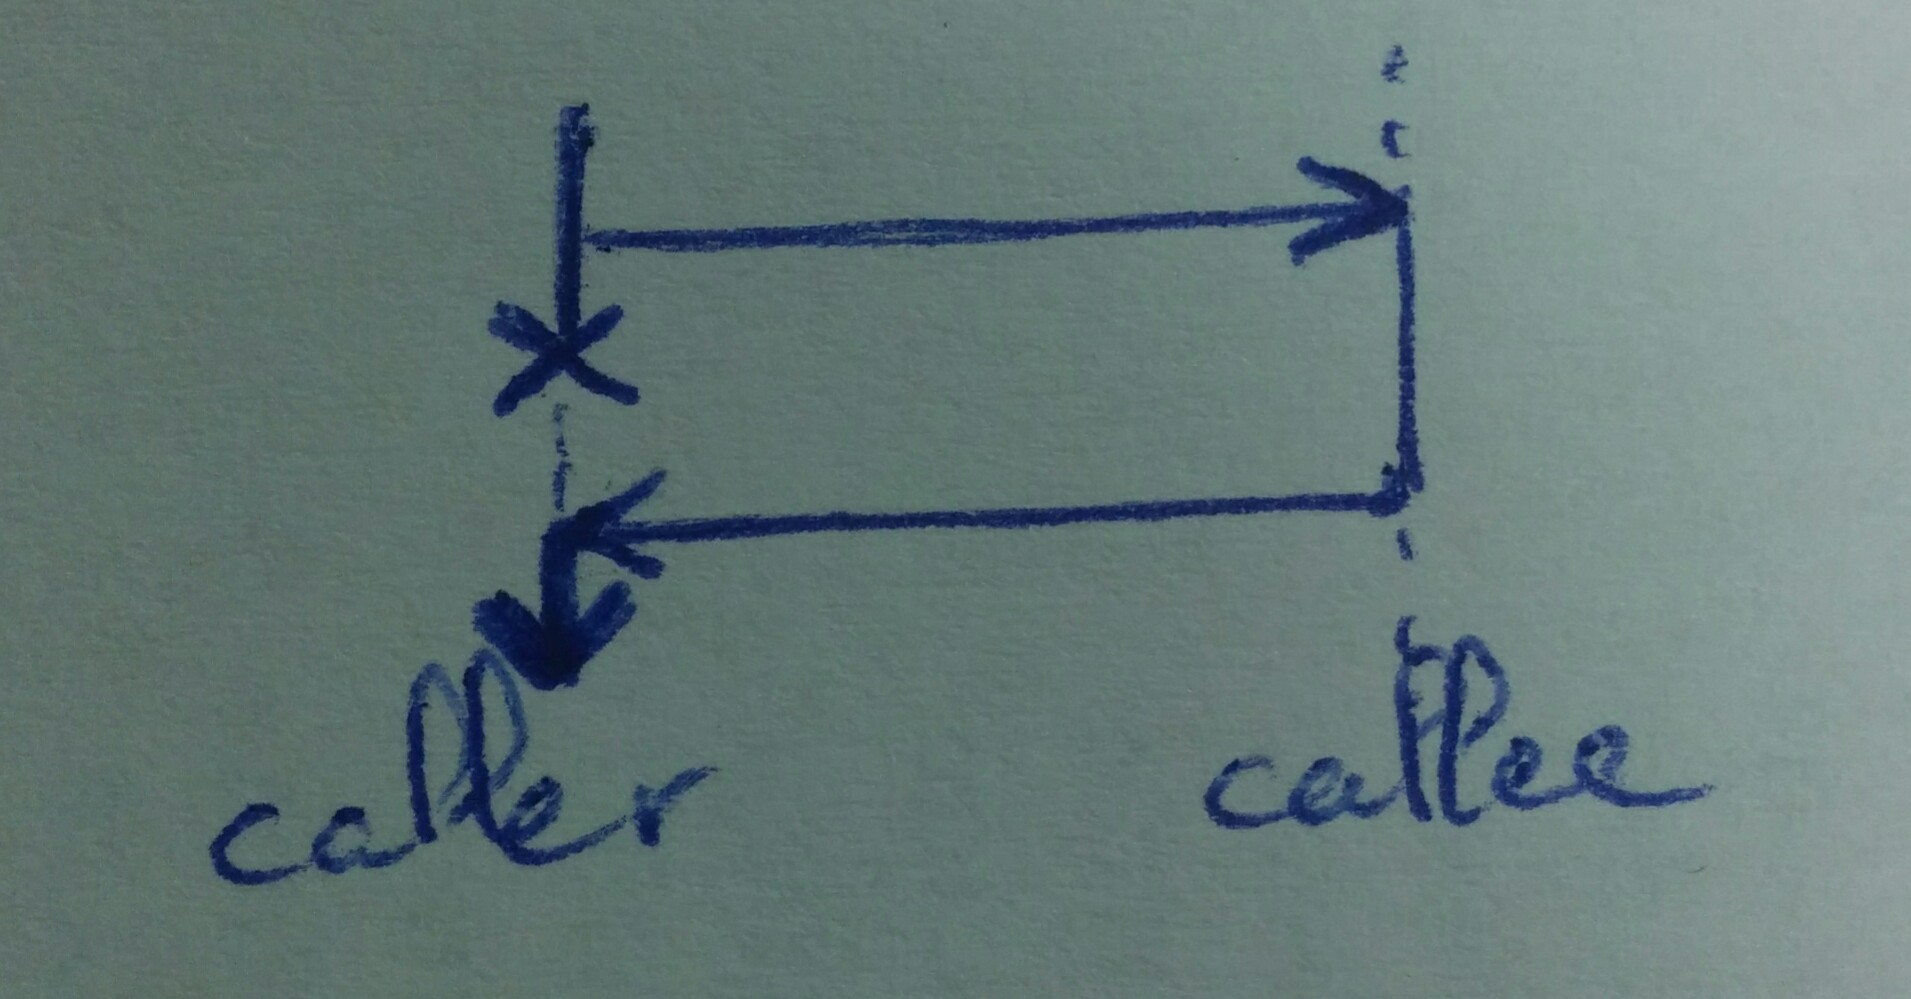
\includegraphics[height=0.2\linewidth]{ressources/block.jpg}
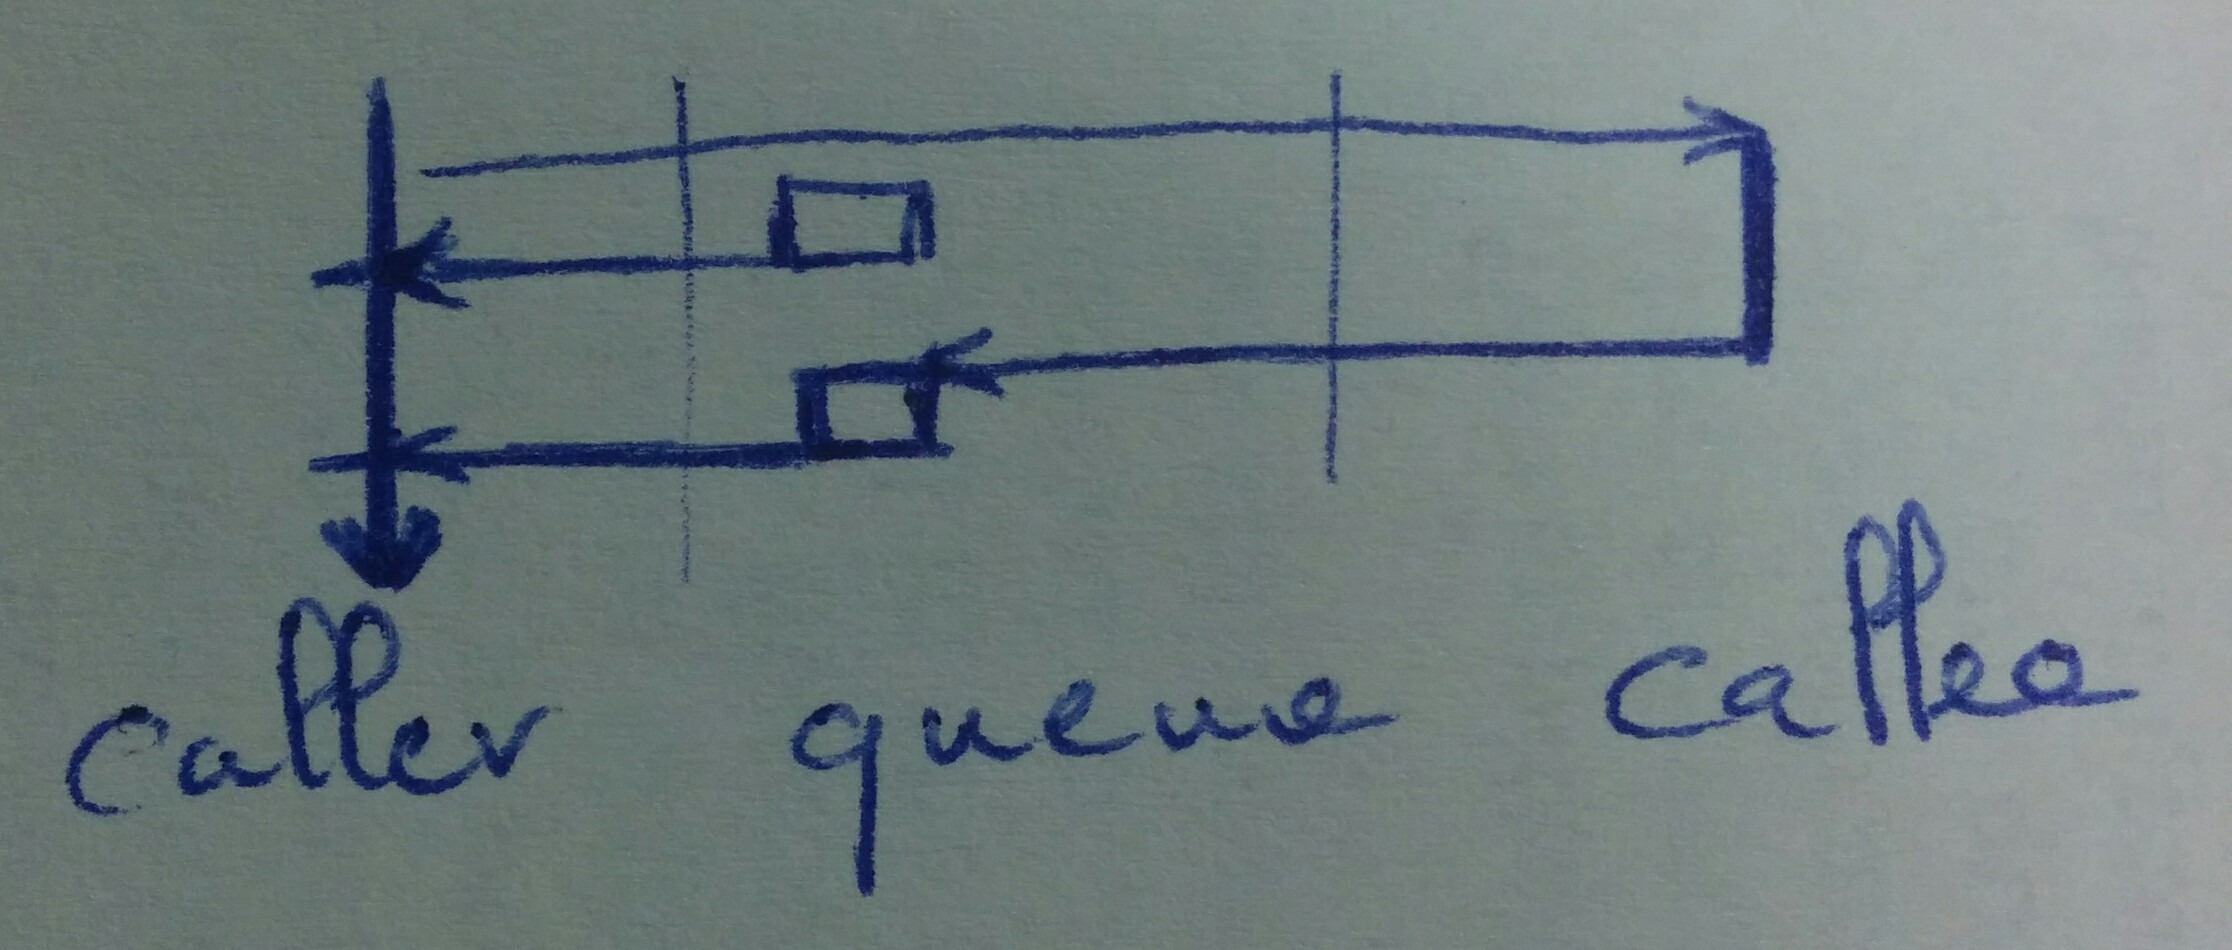
\includegraphics[height=0.2\linewidth]{ressources/queue.jpg}
\caption{Block the execution to wait for the message, or enqueue the message while the execution is available}
\end{center} \end{figure}

For two processes executing concurrently in this asynchronous model, a caller and a callee, we consider two methods of synchronization.
\begin{description}
  \item[The blocking method] reproduces the classical synchronous procedural control flow.
  The caller waits while the function is called.
  In practice, it provides tools making the execution obey the linearity described in the source code.
  The caller wastes computation time waiting for the callee.
  We define this model as a default pessimistic blocking approach that consumes few memory but spends computation time waiting.
  This is the standard approach of many programming language and API. Java threads and IPC are such toolboxes.
  Most of the developers are trained to this programming model.

  \item[The queuing method] breaks the equivalence between source code and the corresponding linear execution.
  The execution part dependent on the result is linked to the asynchronous operation, and is executed only after the completion of the operation.
  It avoids the caller to wait.
  It stores the computed result until it is ready for the caller.
  All the computation results are queued to be processed one at a time by the linked, dependent execution.
  None of the processes waits for the other, but memory usage increases to hold the future results.
  We consider this model as a default running optimistic approach, that optimizes the execution time, but uses more memory.
  This approach is, for example, implemented with a message queue and an event-loop.
  Node.js\footnote{\raggedright http://nodejs.org/}, Ruby EventMachine\footnote{\raggedright http://rubyeventmachine.com/}, Python Twisted\footnote{\raggedright https://twistedmatrix.com/trac/} rely on this paradigm.
\end{description}

While the \textit{blocking method} preserves the determinism of the synchronous computation model, the \textit{queuing method} optimizes the execution time by discarding this determinism.
These two methods are on the opposite ends of a space-time trade-off.
The \textit{blocking method} reduces the memory foot-print and is more suited for a small need for synchronizations.
The \textit{queuing method} reduces the execution time foot-print, and performs well for a large number of short, independent executions using many asynchronous operations.
Web applications fit exactly this second case and use efficiently this method in their implementation.
Network applications are inherently non-deterministic.
The \textit{queuing method} accepts it as its core concept.
It trades determinism for a better scalability.

Web applications manipulate flow of requests ; in this sense, they are very similar to a network router.
Flow of packets are managed with notions like bandwidth, packet size, and quality of service.
It makes sense to use a flow-based language to express web applications - and similar classes of applications.
Many flow-based languages are designed to help an execution model to understand the application as a network of independent actors manipulating flows.
They provide a scalable paradigm to develop highly concurrent applications.
But this approach is orthogonal to the mostly used, imperative approach, and fails to hit a large community of developers.

Thanks to the web browser Javascript programming model, the \textit{queuing method} is growing as an alternate programming model.
Yet it still lacks scalability required for web applications when implemented with a unique event-loop like in \textit{Node.js} or in the browser DOM.
While a flow-based approach is an efficient execution model but fails as a developing language.
We present in this paper an equivalence to link this growing programming model with that scalable execution model.
And allow to build compilers bringing both scalability and the familiarity of the monolithic programming paradigm to web applications in production.

In section \ref{source}, we detail the class of language based on the \textit{queuing method}.
In section \ref{target}, we detail the class of flow-based language.
In section \ref{equivalence}, we develop a set of equivalence between the two classes of language in order to develop a compiler.
In section \ref{test}, we test the performance of our compiler both in terms of development time, and efficiency.
Finally, we conclude this paper.